% !TeX document-id = {beb7ced9-b3cd-42b2-b16a-3ed3c633a1d9}
\documentclass[]             % options: RDPonly, coveronly, nocover
{NASA}                       %   plus standard article class options
%\DeclareRobustCommand{\mmodels}{\mathrel{|}\joinrel\Relbar}

\usepackage[utf8]{inputenc}
\usepackage{csquotes}
\usepackage{setspace}
\usepackage{hyperref}
\usepackage{amsmath, amssymb, amscd, amsthm, amsfonts}
\usepackage{mathtools}
\usepackage{graphicx}
\usepackage{hyperref}
\usepackage{amsthm}
\usepackage[english]{babel}
\usepackage{proof}

\newtheorem{example}{Example}

\newcommand{\B}{\mathbf{B}}
\newcommand{\w}{\mathbf{w}}
\usepackage{proof}
\usepackage{tikz-cd}
\tikzcdset{scale cd/.style={every label/.append style={scale=#1},
		cells={nodes={scale=#1}}}}
\usepackage{stmaryrd}
\hypersetup{
	colorlinks=true,
	linkcolor=blue,
	filecolor=magenta,
	urlcolor=cyan,
	pdftitle={Overleaf Example},
	pdfpagemode=FullScreen,
}
\urlstyle{same}

% Pandoc stuff
\newlength{\cslhangindent}
\setlength{\cslhangindent}{1.5em}
\newlength{\csllabelwidth}
\setlength{\csllabelwidth}{3em}
\newlength{\cslentryspacingunit} % times entry-spacing
\setlength{\cslentryspacingunit}{\parskip}
\newenvironment{CSLReferences}[2] % #1 hanging-ident, #2 entry spacing
 {% don't indent paragraphs
  \setlength{\parindent}{0pt}
  % turn on hanging indent if param 1 is 1
  \ifodd #1
  \let\oldpar\par
  \def\par{\hangindent=\cslhangindent\oldpar}
  \fi
  % set entry spacing
  \setlength{\parskip}{#2\cslentryspacingunit}
 }%
 {}
\usepackage{calc}
\newcommand{\CSLBlock}[1]{#1\hfill\break}
\newcommand{\CSLLeftMargin}[1]{\parbox[t]{\csllabelwidth}{#1}}
\newcommand{\CSLRightInline}[1]{\parbox[t]{\linewidth - \csllabelwidth}{#1}\break}
\newcommand{\CSLIndent}[1]{\hspace{\cslhangindent}#1}


\newtheorem{theorem}{Theorem}[section]
\newtheorem{corollary}{Corollary}[theorem]
\newtheorem{lemma}[theorem]{Lemma}

\theoremstyle{definition}
\newtheorem{definition}{Definition}[section]

\title{Continuous Consistency in the Coordination of
  Airborne and Ground-Based Agents} \author{Lawrence Dunn and Alwyn
  E. Goodloe}

\AuthorAffiliation{Lawrence Dunn \\ Department of Computer and Information
Science \\ University of Pennsylvania \\ Philadelphia, PA \\ Alwyn Goodloe\\                                          % for cover page
  NASA Langley Research Center, Hampton, Virginia
}
\NasaCenter{Langley Research Center\\Hampton, Virginia 23681-2199}
\Type{TM}                    % TM, TP, CR, CP, SP, TT
\SubjectCategory{64}         % two digit number
\LNumber{XXXXX}              % Langley L-number
\Number{XXXXXX}              % Report number
\Month{12}                   % two digit number
\Year{2022}                  % four digit number
\SubjectTerms{Distributed Systems, Formal Methods, Logic, }     % 4-5 comma separated words
\Pages{46}                   % all the pages from the front to back covers
\DatesCovered{}              % 10/2000--9/2002
\ContractNumber{}            % NAS1-12345
\GrantNumber{}               % NAG1-1234
\ProgramElementNumber{}
\ProjectNumber{}             % NCC1-123
\TaskNumber{}                % Task 123
\WorkUnitNumber{}            % 123-45-67-89
\SupplementaryNotes{}
\Acknowledgment{The work was conducted during a summer internship at the NASA Langley Research Center in the Safety-Critical Avionics Systems Branch focusing on distributed computing  issues arising in the Safety Demonstrator challenge in the NASA Aeronautics System Wide Safety (SWS) program.}

%Added for Pandoc
\providecommand{\tightlist}{%
  \setlength{\itemsep}{0pt}\setlength{\parskip}{0pt}}
% Added for subfigures
\usepackage{caption}
\usepackage{subcaption}

\abstract{The System Wide Safety (SWS) program has been investigating
how crewed and uncrewed aircraft can safely operate in shared airspace,
taking disaster response scenarios as a motivating use case. Enforcing
safety requirements for distributed agents requires coordination by
passing messages over a communication network. However, the operating
environment will not admit reliable high-bandwidth communication between
all agents, introducing theoretical and practical obstructions to global
consistency that make it more difficult to maintain safety-related
invariants. This self-contained memo discusses some of the distributed
systems challenges involved in system-wide safety, focusing on the
practical shortcomings of both strong and weak consistency models for
shared memory. Then we survey two \emph{continuous} consistency models
that come from different parts of the literature. Unlike weak
consistency models, continuous consistency models provides hard upper
bounds on the ``amount'\,' of inconsistency observable by clients.
Unlike strong consistency, these models are flexible enough to
accomodate real-world conditions, such as by providing liveness during
brief network partitions or tolerating disagreements between sensors in
a sensor network. We conclude that continuous consistency models are
appropriate for analyzing safety-critical systems that operate without
strong guarantees about network performance.}

\begin{document}
\newpage
\setcounter{tocdepth}{2}
\tableofcontents
\newpage

\hypertarget{introduction}{%
\section{Introduction}\label{introduction}}

Civil aviation has traditionally focused primarily on the efficient and
safe transportation of people and goods via the airspace. Owing to the
application of sound engineering practices and conservative operating
procedures, flying is today the safest mode of transport. The desire not
to compromise this safety makes it challenging to introduce uncrewed
vehicles into the airspace. To that end, the NASA Aeronautics' Airspace
Operations and Safety Program (AOSP) System Wide Safety (SWS) project
has been investigating how crewed and uncrewed aircraft may safely
operate in shared airspace. Wildfire suppression and hurricane relief
are being studied as motivating use cases, in part because the rules for
operating in the US national airspace are typically relaxed during
natural disasters and relief efforts.

Disaster response scenarios present unique challenges for safe
operations. Of fundamental importance is the need for system-wide
coordination in spite of an unpredictable communications environment.
Designing systems that are resilient to these sorts of environments is a
challenge for distributed computing, a subdiscipline of computer
science. This purpose of this memorandum is to enumerate some of the
considerations involved in coordinating air- and ground-based elements
from a distributed computing perspective, identifying challenges,
potential requirements, and frameworks that suggest possible solutions.

Traditionally, civil aviation has employed simple communication patterns
between airborne and ground-based agents and among aircraft. For
instance, aircraft equipped with Automatic Dependent
Surveillance-Broadcast (ADS-B) monitor their location using GPS and
periodically broadcast this information to air traffic controllers and
nearby aircraft. The use cases under consideration demand more
sophisticated coordination schemes between airborne and ground-based
elements to collectively accomplish goals such as navigating safely in
close proximity, delivering resources to remote locations, and
suppressing fires.

Unfortunately, the operating environment cannot generally be expected to
provide reliable, high-bandwidth internet connections that would allow
any group of system nodes to exchange lots of information quickly. For
instance, obstructions like distance, terrain, smoke, and weather mean
we should expect network packets to be dropped or delayed in
unpredictable ways. We also expect the network characteristics to vary
between deployments and to evolve dynamically in time, with connections
varying in strength as agents move around the environment. These factors
make network performance difficult to predict and control.

Weak guarantees about network performance make it difficult to
coordinate distributed agents and offer strong safety guarantees.
So-called strong consistency models, the subject of most of Section
\ref{sec:background}, can enforce strong safety guarantees, but they are
unworkably brittle---they can only be provided under ideal network
conditions unless severe performance penalties are incurred. An
examplary result is Brewer's CAP theorem (Theorem \ref{thm:cap}), which
implies that neither \emph{atomic} nor \emph{sequential} consistency (C)
can be guaranteed by an eventually-available (A) system in the presense
of network partitions (P). Partitions, or transient drops in network
connectivity, are virtually guaranteed to occur in the environments
under consideration. The CAP theorem therefore implies that we cannot
use strong consistency to enforce safety without sacrificing system
performance, meaning the system's ability to respond to clients'
requests in a reasonable amount of time.

On the other hand, weak consistency models such as \emph{causal} and
\emph{eventual} consistency can be provided by real-world systems.
However, these models are too weak to ensure strong safety guarantees.
In particular, they do not bound the overall divergence between two
replicas of a shared data structure, so they provide few assurances
about the mutual consistency of the data observed by different clients.

At face value, the CAP theorem would seem to imply that either
consistency (hence safety) or availability must be sacrificed by
distributed systems deployed in the field. A more nuanced view is that
the theorem observes a fundamental \emph{tradeoff} between consistency
and availability; this tradeoff is amplified by suboptimal network
performance. While the CAP theorem rules out highly idealized systems
that maintain strong consistency and high availability except under
perfect network conditions, it does not inherently rule out systems that
maintain adequate levels of both consistency and performance under
realistic conditions.

What does it mean to have an ``amount'' of consistency? The idea is made
precise by continuous consistency models, or formal measures of
(in)consistency as a continuous value rather than a Boolean condition.
This memo describes two continuous consistency models in the literature.
Both define consistency as an upper bound on the amount of
\emph{inconsistency} between objects, though the models are concerned
with different kinds of objects. One model, the theory of \emph{conits},
comes from research into distributed shared memory. The other,
\emph{sheaf-theoretic data fusion}, comes from research in data
integration and sensor networks. Both define consistency as something
which, in principle, varies smoothly. At one extreme, both models
describe a form of ``perfect'' consistency that cannot usually be
expected in real applications. At the other extreme, the models enforce
no guarantees. In the middle, they place upper bounds on the divergence
between related data objects.

Broadly speaking, it stands to reason that quantitative measurements of
consistency should in turn offer quantitative measurements of safety.
One potential application of having a continuous consistency model is
therefore to compute the amount of safety provided by a deployed system
and enforce this value to within tolerable limits. As we see in Section
\ref{sec:background}, the CAP theorem implies that network performance
can become so poor that a system cannot provide tolerable safety levels
while maintaining availability. When adequate safety margins cannot be
enforced, authorities can decide to take fewer risks. What is centrally
important is to know \emph{how much} safety one has, and that is
(hopefully) what is provided by the models described in this document.

\hypertarget{layout-of-this-document}{%
\subsection{Layout of this document}\label{layout-of-this-document}}

This memo focuses on two (prima facie unrelated) notions of continuous
consistency developed in the literature. This document aims to be
reasonably self-contained and readable to a broad technical audience. It
is laid out as follows.

Section \ref{sec:background} provides a high-level introduction to
distributed systems and memory consistency models. We define two strong
models, atomic and sequential consistency, both of which provide highly
desirable safety guarantees; we contrast these with the weaker
guarantees implied by the causal consistency model. Then we turn our
attention to the CAP theorem (Brewer 2000) (Gilbert and Lynch 2002),
which captures a fundamental consistency/availability tradeoff in the
presense of network partitions. We observe that the theorem effectively
prohibits both forms of strong consistency in our intended use case.
This raises the question of how, if at all, one can rigorously enforce
safety properties without compromising system performance beyond
acceptable levels.

Informed by the previous discussion, Section \ref{sec:des} offers a list
of three desiderata of distributed applications in the contexts under
consideration. These have been selected as especially desirable and
relevant for our use cases, and they provide a basis for assessing the
applicability of frameworks and techniques to overcome the apparent
limitations imposed by the CAP theorem.

Section \ref{sec:contcons} explains how the \emph{conit} framework (Yu
and Vahdat 2002) quantifies the C/A tradeoff with respect to three
metrics: numerical error, order commit error, and real-time error. We
summarize how to enforce consistency up to some real-valued
\(\epsilon \geq 0\) for each of these metrics separately. The conit
framework allows applications to specify their own consistency semantics
with respect to these measurements, and to mark updates as having a
greater or lesser impact on consistency. Each replica, indeed each
system request, can set its own bounds on observable inconsistency,
while a general-purpose middleware library transparently enforces these
requirements. At the extreme, the framework can enforce either atomic or
sequential consistency by setting \(\epsilon = 0\) for
appropriately-defined conits. For \(\epsilon > 0\), the framework offers
neither CAP-consistency nor CAP-availability; in return, applications
can provide limited amounts of availability, possibly during network
partitions, while strictly bounding levels of inconsistency. One use
case for this is to ``smooth out'' intermittent fluctuations in network
performance, a desirable feature for safety-critical systems operating
without strict assumptions about the network.

Section \ref{sec:sheaf} is an introduction to applied sheaf theory,
which provides a highly general framework for measuring the mutual
consistency of ``overlapping'' observations. Intuitively, these are
observations which we expect to be correlated if not equal, such as the
data generated by nearby sensors in a sensor network. We discuss an
simulated example, due to (Robinson 2017), where sheaves are used to
integrate heterogeneous sensor data, thereby improving an estimated
location for a crashed aircraft. Unlike many introductions to the
subject, we emphasize sheaves as ``topologically-flavored'' presheaves,
viewing presheaves as highly generalized transition systems. Our
expectation is that this approach makes the subject more accessible to
computer scientists and serves to highlight themes common to Sections
\ref{sec:contcons} and \ref{sec:sheaf}. It may even indicate the
possibility of re-grounding conit theory in the principled mathematical
framework of sheaf theory.

Section \ref{sec:conclusion} concludes with suggestions for future work.

\hypertarget{distributed-systems}{%
\section{Distributed systems}\label{distributed-systems}}

\hypertarget{distributed-systems-1}{%
\section{Distributed systems}\label{distributed-systems-1}}

\label{sec:background}

A distributed system, broadly construed, is a collection of independent
entities that cooperate to solve a problem that cannot be individually
solved (Kshemkalyani and Singhal 2008). In the context of computing,
(Singhal and Shivaratri 1994) offer the following definition.

\begin{quote}
``A collection of computers that do not share common memory or a common
physical clock, that communicate by message passing over a communication
network, and where each computer has its own memory and runs its own
operating system.''
\end{quote}

A fundamental goal for distributed computing systems is to
``{[}appear{]} to the users of the system as a single coherent
computer'' (Tanenbaum and Steen 2007). This can be understood as the
requirement that all nodes present a \emph{mutually-consistent} view of
the world, e.g.~the state of a globally-maintained database, to system
clients.

When \emph{strong consistency} is enforced, clients cannot tell whether
they are all interacting with a single central computer, or a complex
system of independent computers acting in tandem. This abstraction
shields clients and application developers from complexity and makes it
simpler to reason about system behavior. For example, if a client
modifies a data structure by submitting a write request to one system
node, a strongly consistent system must ensure that other nodes reflect
the update as well. If some nodes were to reflect the update while
others did not, the abstraction of a shared world would be broken, the
clients' mental model of the system can become invalid, and safety
requirements may be violated. A few examples of the perils of
inconsistency:

\begin{itemize}
\item
  A bank client would be unhappy if deposits that appear in their
  account online are not reflected when they check their balance at an
  ATM, or if they disappear after refreshing the webpage.
\item
  Air traffic controllers cannot safely coordinate the movement of
  aircraft if they are presented with conflicting or out-of-date
  information about their positions and velocities.
\item
  Potentially dangerous misunderstandings can arise in a group messaging
  application if messages appear in different orders to different
  clients.
\item
  Resource-tracking systems cannot be trusted if they do not reflect the
  true information about the availability and location of resources.
\end{itemize}

What exactly constitutes consistency? There are different consistency
models, and the most appropriate model for an application depends on the
semantics it expects, which must be weighed against other requirements.
All other things being equal, one wants to have as much consistency as
possible. Below, we shall see that \textrm{na\"ive} notions of system
coherence are brittle in the sense that they generally cannot be
guaranteed for theoretical and practical reasons; that is, unless one is
willing to pay with significant performance penalties, including
applications that fail to respond to users under some conditions.
Therefore, real-world applications must tolerate weaker notions of
consistency. This makes applications more difficult to reason about, as
their behavior may depend on uncontrollable factors in the environment.
As fewer behaviors can be ruled out, it becomes more difficult to ensure
the system maintains safety-related invariants.

The difficulty of enforcing strong consistency is that it requires
system nodes to coordinate by exchanging information. Absence of a
common memory implies that inter-process communication takes place over
the network (whereas processes on the same machine have the option to
share data by writing it to a common memory location). A foundational
assumption of distributed systems, and an especially apt one in the
context of disaster response scenarios, is that the network is less than
perfectly reliable. Message delivery is not instantaneous, and delivery
times may be unpredictable. The network may be allowed to silently drop
network packets, reorder them, or deliver them several times. In the
case of \emph{Byzantine faults} (CITE) the network may even act like a
malicious adversary (though we will not consider this scenario in this
document). Imperfections in communications represent obstructions to
system consistency and make it challenging to enforce safety
requirements.

We shall now make this discussion more precise by introducing formal
definitions.

\hypertarget{system-model}{%
\subsection{System model}\label{system-model}}

A distributed system consists of a set
\(\mathcal{P} = \{P_i\}_{i\in I}\) of \emph{processes}, which we think
of these as executing on independent, often geographically dispersed
computers that communicate by message-passing.

Process take requests from clients, such as to read or write a value in
a database. The lifecycle of a typical request is depicted in Figure
\ref{fig:request}. At some physical time (i.e.~wall-clock time)
\(C.s \in \mathbb{R}\) (client start time), a client sends a message to
a process. At time \(E.s\), which we'll call the \emph{start time} of
the event, the message is accepted by the process. The request is
processed until some strictly greater time \(E.t > E.s\) when a response
is sent back to the client. The value \(E.t - E.s\) is the
\emph{duration} of the event.

\begin{figure}
  \center
  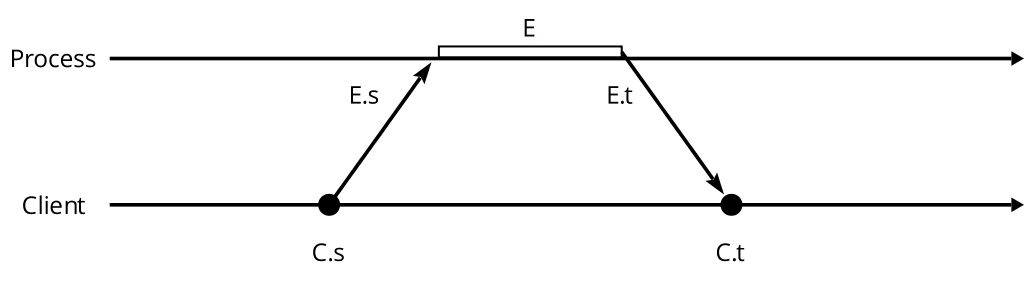
\includegraphics[scale=0.4]{images/request.png}
  \caption{Lifetime of a client request}
  \label{fig:request}
\end{figure}

While handling the request, the process may coordinate with other
processes in the background by sending and receiving more messages. For
example, the process may propagate the client's request to other
processes, retrieve up-to-date values from other processes to give to
the client, or delay handling the client's request in order to handle
other requests.

To discuss consistency models, we shall be less interested in the
details of message-passing and more interested just in the responses
observed by clients. We shall consider the full set of events across a
distributed system, such as shown in Figure \ref{fig:externalorder}.
This is called an \emph{execution}. Consistency models constrain the set
of allowable return values in response to clients' requests.

As is often the case, we shall assume that requests handled by a single
process do not overlap in time. This can be enforced with local
serialization methods such as two-phase locking (CITE) that can be used
to isolate concurrent transactions from each other, providing the
abstraction of a system that handles requests one at a time. On the
other hand, any two processes may handle two events at the same physical
time, so that there is no obvious total order of events across the
system. Instead, one has a partial order called \emph{external order}.
Intuitively, it is the partial order of events that would be witnessed
by an observer recording the real time at which systems begin and finish
responding to requests.

\begin{definition}
Let $E$ be an execution. Request $E1$ \emph{externally precedes}
request $E2$ if $E1.t < E2.s$. That is, if the first request
terminates before the second request is accepted. This induces an
irreflexive partial order called \emph{external order}.
\end{definition}

Recall that an irreflexive partial order is a binary relation \(<\) such
that \(A \not < A\), \(A < B \implies B \not < A\), and
\(A < B, B < C \implies A < C\).

Because we assume processes handle events one-at-a-time, the events
handled at any one process are totally ordered by external order---one
event cannot start before another has finished. If \(E1\) and \(E2\) are
events at \emph{different} processes, they need not be comparable by
external order, i.e.~neither \(E1.t < E2.s\) nor \(E2.t < E1.s\), making
them \emph{physically concurrent}.

\begin{definition}
If two events overlap in physical time
(equivalently, if they are not comparable by external order), we call the events \emph{physically concurrent} and
write $E1 || E2$.
\end{definition}

Physical concurrency is a reflexive and symmetric---but usually not
transitive--- binary relation. Such structures are often called
\emph{compatibility relations.} The general intuition is that anything
is compatabile with itself (reflexivity), and the compatibility of two
objects does not depend on their order (symmetry). But if \(A\) and
\(B\) are compatible with \(C\), it need not be the case that \(A\) and
\(B\) are compatible with each other.

Figure \ref{fig:externalorderexec} shows the external order relation for
an execution. To save space we elide arrows between two events of the
same process and arrows that can be inferred by transitivity. This
corresponds to the directed acyclic graph structure shown in
\ref{fig:externalorderdag}.

\begin{figure}
     \begin{subfigure}[a]{1\textwidth}
         \center
         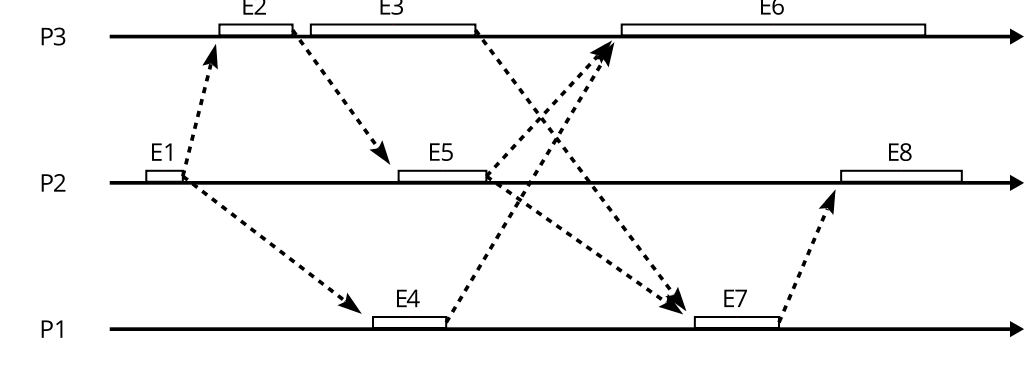
\includegraphics[scale=0.4]{images/externalorder.png}
         \caption{Depiction of external order between concurrent events across three processes. Intra-process and transitive edges are not depicted.}
         \label{fig:externalorderexec}
     \end{subfigure}
     \begin{subfigure}[b]{1\textwidth}
         \center
         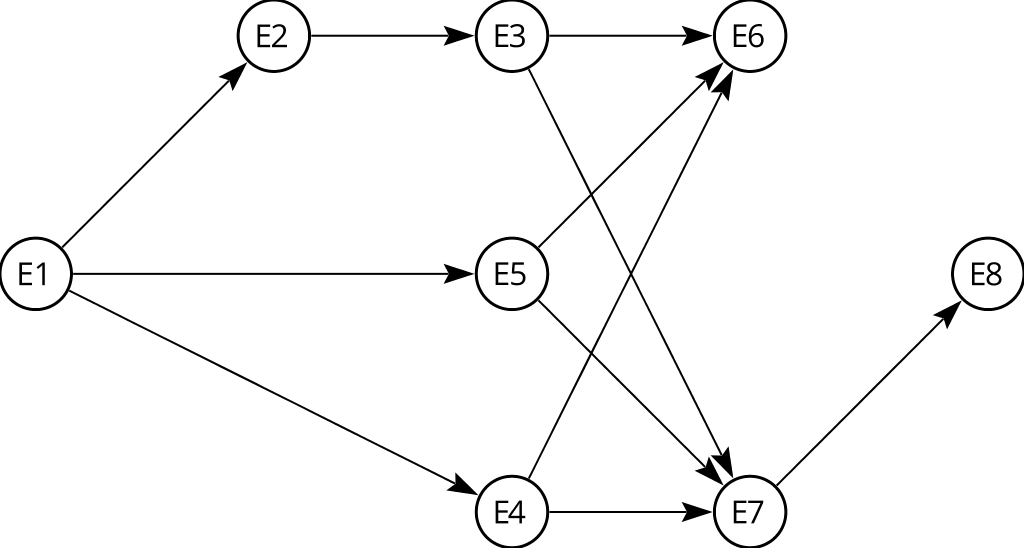
\includegraphics[scale=0.25]{images/partialorder.png}
         \caption{The directed acyclic graph (DAG) induced by external order.}
         \label{fig:externalorderdag}
     \end{subfigure}
     \caption{External order}
     \label{fig:externalorder}
\end{figure}

The reader may wonder if we can consider events to be totally ordered,
say by pairing them with a timestamp that records their physical start
time to resolve ties like \(x || y\). This order is not generally useful
for a couple reasons. First, we assume processes have only loosely
synchronized clocks, so timestamps from two different processes may not
be comparable. Additionally, even systems that enforce linearizable
consistency (c.f. Section \ref{sec:atomic}) do not necessarily handle
requests in order of their physical start times.

\hypertarget{linearizability-and-the-cap-theorem}{%
\subsection{Linearizability and the CAP
theorem}\label{linearizability-and-the-cap-theorem}}

\label{sec:atomic}

A fundamental distributed application is the \emph{shared distributed
memory} abstraction. We shall assume that all processes maintain a local
replica of a globally shared data object, as replication increases
system fault tolerance. For simplicitly, we shall discuss the data store
as a simple key-value store, but it could be something else like a
database, filesystem, persistent object, etc.

We assume clients submit two types of requests to processes. A
\emph{read request} is a request to lookup the current value of a
variable. A request to read the variable \(x\) that returns value \(a\)
is written \(R(x,a)\). A \emph{write request} is a request to set the
current value of a variable. Notation \(W(x,a)\) represents writing
value \(a\) to \(x\). We assume all processes provide access to the same
set of shared variables.

A \emph{memory consistency model} formally constrains the allowable
system responses during executions. \emph{Strong} consistency models are
generally understood as ones provide the illusion that all clients are
accessing just one globally shared replica. As we will see, this still
leaves room for different possible behaviors (i.e.~allows
non-determinism in the execution of a distributed application), but the
allowable behavior is tightly constrained.

\emph{Linearizability} (Herlihy and Wing 1990) is essentially the
strongest common consistency model. It is known variously as atomic
consistency, strict consistency, and sometimes external consistency. In
the context of database transactions (which come with other guarantees,
like isolation, that are more specific to databases), the analogous
condition is called strict serializability. A linearizable execution is
defined by three features:

\begin{itemize}
\tightlist
\item
  All processes act like they agree on a single, global total order
  defined across all accesses.
\item
  This sequential order is consistent with the actual external order.
\item
  Responses are semantically correct, meaning a read request \(R(x, a)\)
  returns the value of the most recent write request \(W(x, a)\) to
  \(x\).
\end{itemize}

We can also phrase this in terms of \emph{linearizations.}

\begin{definition}
A \emph{linearization point} $t \in \mathbb{R} \in [E.s, E.t]$ for an
event $E$ is a time between the event's start and termination. An
execution is \emph{linearizable} if and only if there is a choice of
linearization point for each access, which induces a total order called a \emph{linearization},
such that $E$ is equivalent to
the serial execution of events when totally ordered by their
linearization points.
\end{definition}

Intuitively, it should appear to an external observer that each access
instantaneously took effect at some point between its start and end
time. It is assumed no distinct access can have the same linearization
point, so that we get a total order. We say an entire system is
linearizable when all possible executions of the system are
linearizable.

Figure \ref{fig:linear_example11} shows a prototypical example of a
linearizable execution. We assume that all memory locations are
initialized to \(0\) at the system start time. Figure
\ref{fig:linear_example12} shows an execution that is not linearizable
because the read access on \(y\) on \(P1\) returns stale data instead of
reflecting the write access to \(y\) on \(P2\).

\begin{figure}
     \begin{subfigure}[a]{1\textwidth}
         \center
         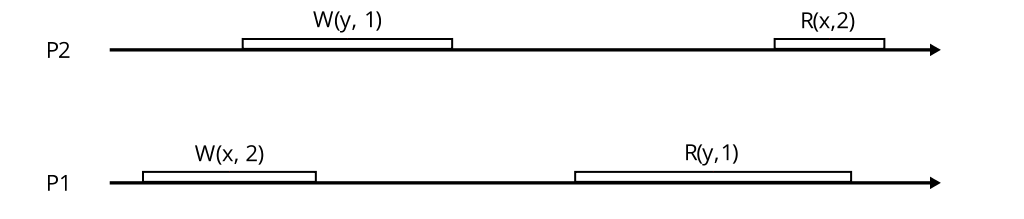
\includegraphics[scale=0.4]{images/linear1.png}
         \caption{A linearizable execution. Any choice of linearization works here.}
         \label{fig:linear_example11}
     \end{subfigure}
     \begin{subfigure}[b]{1\textwidth}
         \center
         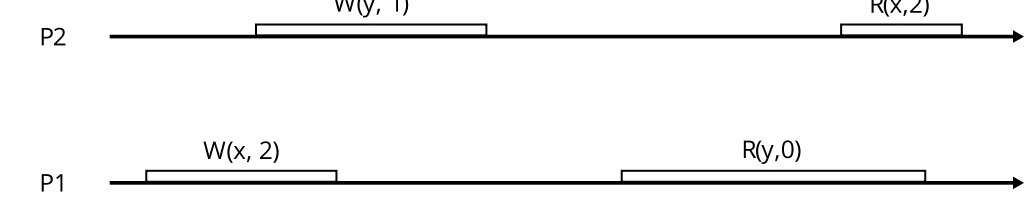
\includegraphics[scale=0.4]{images/nonlinear0.png}
         \caption{A non-linearizable execution. The request to read $y$ returns a stale value. }
         \label{fig:linear_example12}
     \end{subfigure}
  \caption{A linearizable and non-linearizable execution.}
  \label{fig:linear_example1}
\end{figure}

Linearization points are demonstrated in Figure \ref{fig:linearization}.
The figure shows different linearizable behaviors in response to the
same underlying set of accesses. This demonstrates that linearizability
still leaves some room for non-determinism in the execution of
distributed applications. In this example, the requests must both return
1 or 2. The constraint is that the values must agree---linearizability
forbids the situation in which one client reads \(1\) and another reads
\(2\) (Figure \ref{fig:nonlinearizable}).

\begin{figure}
     \begin{subfigure}[a]{1\textwidth}
         \center
         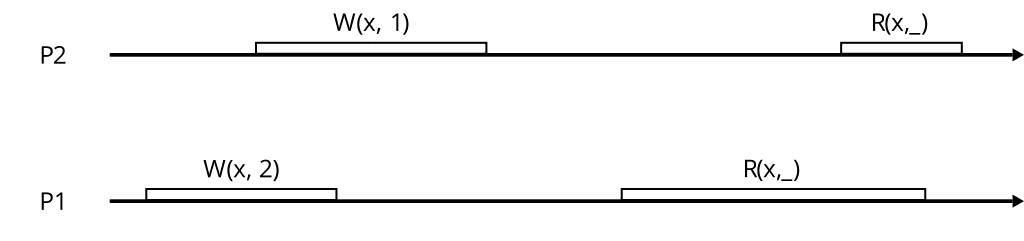
\includegraphics[scale=0.4]{images/linearTemplate.png}
         \caption{An execution with read responses left unspecified.}
         \label{fig:nonlinear}
     \end{subfigure}
     \begin{subfigure}[b]{1\textwidth}
         \center
         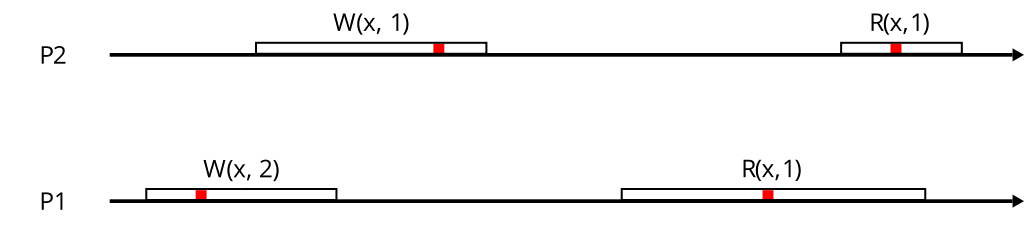
\includegraphics[scale=0.4]{images/linear3.png}
         \caption{A linearizable execution for which both reads return $1$.}
     \end{subfigure}
     \begin{subfigure}[c]{1\textwidth}
         \center
         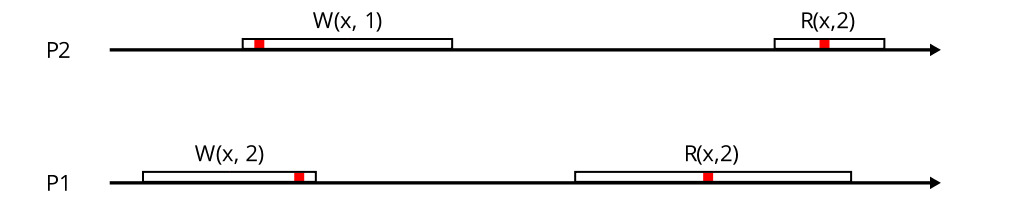
\includegraphics[scale=0.4]{images/linear2.png}
         \caption{A linearizable execution for which both reads return $2$.}
     \end{subfigure}
  \caption{Two linearizable executions of the same underlying events that return different responses. Possible linearization points are shown in red.}
  \label{fig:linearization}
\end{figure}

\begin{figure}
     \begin{subfigure}[a]{1\textwidth}
         \center
         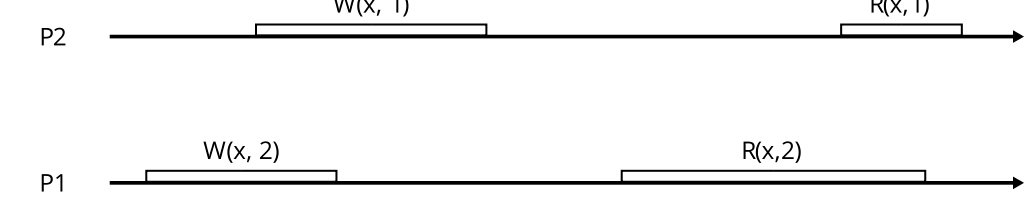
\includegraphics[scale=0.4]{images/nonlinear1.png}
         \caption{A nonlinearizable execution with the read access returning disagreeing values. We will see later (Figure \ref{fig:sequential}) that this execution is still sequentially consistent. }
         \label{fig:nonlinear1}
     \end{subfigure}
     \begin{subfigure}[b]{1\textwidth}
         \center
         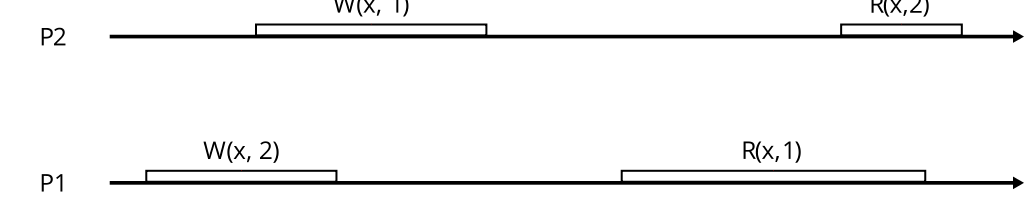
\includegraphics[scale=0.4]{images/nonlinear2.png}
         \caption{Another nonlinearizable execution with read access values swapped. This execution is not sequentially consistent.}
         \label{fig:nonlinear2}
     \end{subfigure}
  \caption{Two non-linearizable executions of the same events shown in Figure \ref{fig:linearization}.}
  \label{fig:nonlinearizable}
\end{figure}

\hypertarget{enforcing-linearizability}{%
\paragraph{Enforcing linearizability}\label{enforcing-linearizability}}

Linearizability can be enforced with a total order broadcast mechanism
(CITE). Total order broadcast is a means for processes to come to a
consensus about the order of a set of events. One can imagine that the
total order broadcast API implements a routine that accepts a message
and notifies all other processes of this message in such a way that all
processes see all messages in the same order. To maintain
linearizability, it suffices that each replica applies database actions
in the order they are announced in the total order broadcast. A subtle
point is that a process does not need to handle read requests originally
sent to other clients, so these may be ignored. However, the originating
replica must not handle its own read requests until \emph{after} they
appear in the total order broadcast, rather than at the time they are
first submitted to the total order broadcast mechanism.

\hypertarget{the-cap-theorem}{%
\subsubsection{The CAP Theorem}\label{the-cap-theorem}}

Real-world systems often fall short of behaving as a single perfectly
coherent system. The root of this phenomenon is a deep and
well-understood tradeoff between system coherence and performance.
Enforcing consistency comes at the cost of additional communications,
and communications impose overheads, often unpredictable ones.

Fox and Brewer (Fox and Brewer 1999) are crediting with observing a
particular tension between the three competing goals of consistency,
availability, and partition-tolerance. This tradeoff was precisely
stated and proved in 2002 by Gilbert and Lynch (Gilbert and Lynch 2002).
The theorem is often somewhat misunderstood, as we discuss, so it is
worth clarifying the terms used.

\hypertarget{consistency}{%
\paragraph{Consistency}\label{consistency}}

Gilbert and Lynch define a consistency system as one whose executions
are always linearizable.

\hypertarget{availability}{%
\paragraph{Availability}\label{availability}}

A CAP-available system is one that will definitely respond to every
client request at some point.

\hypertarget{partition-tolerance}{%
\paragraph{Partition tolerance}\label{partition-tolerance}}

A partition-tolerant system continues to function, and ensure whatever
guarantees it is meant to provide, in the face of arbitrary partitions
in the network (i.e., an inability for some nodes to communicate with
others). It is possible that a partition never recovers, say if a
critical communications cable is permanently severed.

A partition-tolerant CAP-available system cannot indefinitely suspend
handling a request to wait for network activity like receiving a
message. In the event of a partition that never recovers, this would
mean the process could wait indefinitely for the partition to heal,
violating availability. On the other hand, a CAP-consistent system is
not allowed to return anything but the most up-to-date value in response
to client requests. Keep in mind that any (other) process may be the
originating replica for an update. Some reflection shows that the full
set of requirements is unattainable---a partition tolerant system simply
cannot enforce both consistency and availability.

\begin{theorem}[The CAP Theorem]
    \label{thm:cap}
    In the presense of indefinite network partitions, a distributed system
    cannot guarantee both linearizability and eventual-availability.
\end{theorem}
\begin{proof}
Technically, the proof is almost trivial. We give only the informal
sketch here, leaving the interested reader to consult the more formal
analysis by Gilbert and Lynch. The key technical assumption is that a
processes' behavior can only be influenced by the messages it actually
receives---it cannot be affected by messages that are sent to it but
never delivered.

In Figure \ref{fig:linear_example11}, suppose the two processes are on
opposite sides of a network partition, so that no information can be
exchanged between them (even indirectly through a third party). If we
just consider the execution of $P_2$ by itself, without $P_1$,
linearizability would require it to read the value $2$ for $y$. If we
do consider $P_1$, linearizability requires that the read access to
$y$ must return $1$. But if $P_2$ cannot send messages to $P_1$, then
$P_2$'s behavior cannot be influenced by the write access to $y$, so
it would still have to return $2$, violating
consistency. Alternatively, it could delay returning any result until
it is able to exchange messages with $P_1$. But if the partition never
recovers, $P_1$ will wait forever, violating availability.
\end{proof}

While the proof of the CAP theorem is simple, its interpretation is
subtle and has been the subject of much discussion in the years since
(Brewer 2012). It is sometimes assumed that the CAP theorem claims that
a distributed system can only offer two of the properties C, A, and P.
In fact, the theorem constrains, but does not prohibit the existence of,
applications that apply some relaxed amount of all three features. The
CAP theorem only rules out their combination when all three are
interpreted in a highly idealized sense.

In practice, applications can tolerate much weaker levels of consistency
than linearizability. Furthermore, network partitions are usually not as
dramatic as an indefinite communications blackout. Real conditions in
our context are likely to be chaotic, featuring many smaller disruptions
and delays and sometimes larger ones. Communications between different
clients may be affected differently, with nearby agents generally likely
to have better communication channels between them than agents that are
far apart. Finally, CAP-availability is a suprisingly weak condition.
Generally one cares about the actual time it takes to handle user
requests, but the CAP theorem exposes difficulties just ensuring the
system handles requests at all. Altogether, the extremes of C, A, and P
in the CAP theorem are not the appropriate conditions to apply to many,
perhaps most, real-world applications.

Broadening our perspective, the tension between consistency and
availability is a prototypical example of a deeper tension in computing:
that between safey and liveness properties (Davidson, Garcia-Molina, and
Skeen 1985; Gilbert and Lynch 2012). These terms can be understood as
follows.

\begin{itemize}
\item
  \textbf{Safety} properties ensure that a system avoids doing something
  ``bad'\,' like violating a consistency invariant. Taken to the
  extreme, one way to ensure safety is to do nothing. For instance, we
  could enforce safety by never responding to read requests in order to
  avoid offering information that is inconsistent with that of other
  nodes.
\item
  \textbf{Liveness} properties ensure that a system will eventually do
  something ``good'\,', like respond to a client. Taken to the extreme,
  one very lively behavior would be to immediately respond to user
  requests, without taking any steps to make sure this response is
  consistent with that of other nodes.
\end{itemize}

Note that in our use cases, an unresponsive system could arguably be
``unsafe.'' The distinction between the terms in this narrow context is
that ``safety'' constrains a system's allowable responses to clients, if
one is even given, while liveness requires giving responses. The fact
that both of these have implications for human safety is one more reason
to prefer continuous consistency models over CAP-unavailabile models
like linearizability.

Because of the tension between them, building applications that provide
both safety and liveness features is challenging. The fundamental
tradeoff is that if we want to increase how quickly a system can respond
to requests, eventually we must relax our constraints on what the system
is allowed to return.

Next we consider a slightly more relaxed consistency model that admits a
greater range of system behaviors while maintaining the total order
guarantees of atomic consistency.

\hypertarget{sequential-consistency}{%
\subsection{Sequential consistency}\label{sequential-consistency}}

\begin{figure}
     \begin{subfigure}[a]{1\textwidth}
         \center
         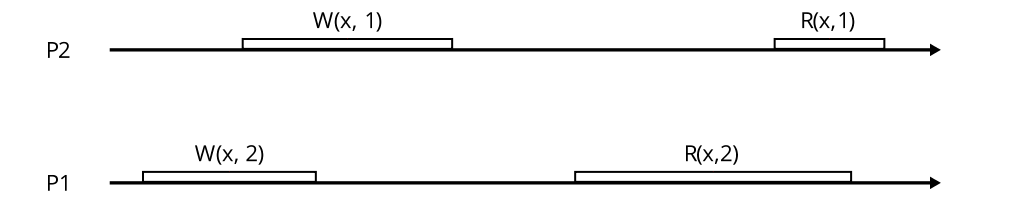
\includegraphics[scale=0.4]{images/sequential1.png}
         \caption{A non-linearizable, sequentially consistent execution.}
         \label{fig:sequential1}
     \end{subfigure}
     \begin{subfigure}[b]{1\textwidth}
         \center
         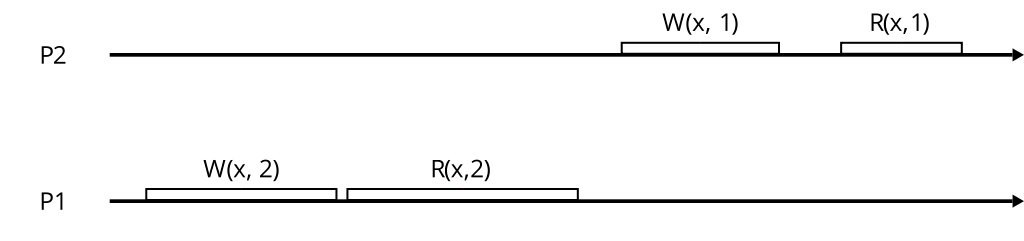
\includegraphics[scale=0.4]{images/sequential2.png}
         \caption{An equivalent interleaving of \ref{fig:sequential1}.}
         \label{fig:interleaving1}
     \end{subfigure}
     \caption{A sequentially consistent execution and a possible interleaving.}
     \label{fig:sequential}
\end{figure}

Enforcing atomic consistency means that an access \(E\) at process
\(P_i\) cannot return to the client until every other process has been
informed about \(E\). For many applications this is an unacceptably high
penalty. A weaker model that is still strong enough for most purposes is
\emph{sequential} consistency. This is an appropriate model if a form of
strong consistency is required, but the system is agnostic about the
precise physical time at which events start and finish, provided they
occur in a globally agreed upon order.

A sequentially consistent system ensures that any execution is
equivalent to some global serial execution, even if this is serial order
is not the one suggested by the real-time ordering of events. When
real-time constraints are not important, this provides essentially the
same benefits as linearizability. For example, it allows programmers to
reason about concurrent executions of programs because the result is
always guaranteed to represent some possible interleaving of
instructions, never allowing instructions from one program to execute
out of order.

Processes in a sequentially consistent system are required to agree on a
total order of events, presenting the illusion of a shared database from
an application programmer's point of view. However, this order need not
be given by external order. Instead, the only requirement is that
sequential history must agree with process order, i.e.~the events from
each process must occur in the same order as in they do in the process.

\begin{definition}
\label{def:sequentiallyconsistent}
A \emph{sequentially consistent} execution is
characterized by three features:
\begin{itemize}
\item All processes act like they agree on a single, global total order
  defined across all accesses.
\item This sequential order is consistent with the program order of each process.
\item Responses are semantically correct, meaning reads return the most recent writes (as determined by the global order)
\end{itemize}
\end{definition}

This is nearly the definition of linearizability, except that external
order has been replaced with merely program order. We immediately get
the following lemma.

\begin{lemma}
\label{lem:linearsequential}
    A linearizable execution is sequentially consistent.
\end{lemma}
\begin{proof}
This follows because process order is a subset of external order.
\end{proof}

Visually, sequential consistency allows reordering an execution by
sliding events along each process' time axis like beads along a string.
Two events from the same process cannot pass over each other as this
would violate program order, but events on different processes may be
commuted past each other, violating external order. This sliding allows
defining an arbitrary interleaving of events, a totally ordered
execution with no events overlapping. From this perspective, while
linearizability requires the existence of a linearization, sequential
consistency requires the existence of an equivalent interleaving.

The converse of Lemma \ref{lem:linearsequential} does not hold. For
example, Figure \ref{fig:sequential1} was previously shown (Figure
\ref{fig:nonlinear1}) as a nonlinearizable execution. However, it is
sequentially consistent, as evidenced by the interleaving in Figure
\ref{fig:interleaving1} that slides the events \(W(x,1)\) and \(R(x,2)\)
past each other.

\begin{figure}
     \begin{subfigure}[a]{1\textwidth}
         \center
         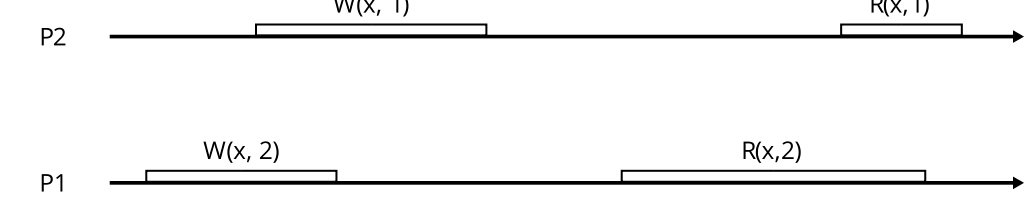
\includegraphics[scale=0.4]{images/nonsequential1.png}
         \caption{A non-sequentially consistent execution.}
         \label{fig:nonsequential1}
     \end{subfigure}
     \begin{subfigure}[b]{1\textwidth}
         \center
         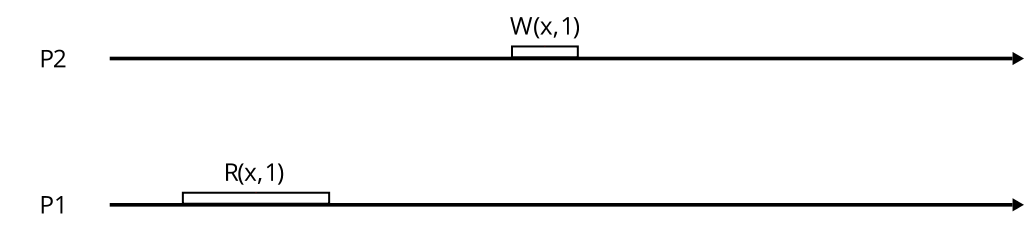
\includegraphics[scale=0.4]{images/nonsequential_x.png}
         \caption{The sequentially consistent history of $x$.}
         \label{fig:sequentialx}
     \end{subfigure}
     \begin{subfigure}[b]{1\textwidth}
         \center
         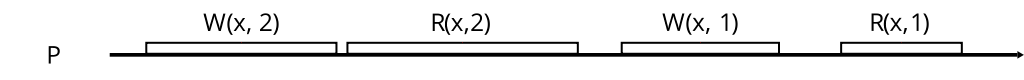
\includegraphics[scale=0.4]{images/nonsequential_y.png}
         \caption{The sequentially consistent history of $y$.}
         \label{fig:sequentialy}
     \end{subfigure}
     \caption{A non-sequentially consistent execution with sequentially-consistent executions at each variable.}
     \label{fig:nonsequential}
\end{figure}

\hypertarget{enforcing-sequential-consistency}{%
\paragraph{Enforcing sequential
consistency}\label{enforcing-sequential-consistency}}

Notably, to enforce sequential consistency for the whole system, it is
not enough to enforce it at the level of individual variables. Figure
\ref{fig:nonsequential1} shows a history that is not sequentially
consistent. However, the histories of accesses to individual variables
(Figures \ref{fig:sequentialx} and \ref{fig:sequentialy}) \emph{are}
sequentially consistent. This is a key difference from linearizability
(CITE).

Like linearizability, sequential consistency can also be enforced with a
total order broadcast mechanism. All write requests are first broadcast,
and replicas only apply updates in the order they appear in the total
order broadcast. The crucial difference from linearizability is that
each process can handle requests immediately, returning its local
replica value, instead of waiting for the broadcast mechanism to assign
a global order to the read request.

\hypertarget{cap-unavailability}{%
\paragraph{CAP unavailability}\label{cap-unavailability}}

Sequential consistency is a relaxation of atomic consistency, but not by
much. The model is still too strict to enforce under partition
conditions.

\begin{lemma}
    An eventually-available system cannot provide sequential consistency in the presense of network partitions.
\end{lemma}
\begin{proof}

The proof is an adaptation of Theorem \ref{thm:cap}. Suppose $P_1$ and
$P_2$ form of CAP-available distributed system and consider the
following execution: $P_1$ reads $x$, then assigns $y$ the value
$1$. $P_2$ reads $y$, then assigns $x$ the value $1$. (Note that this
is the sequence of requests shown in Figure \ref{fig:nonsequential1},
but we make no assumptions about the values returned by the read
requests). By availability, we know the requests will be handled (with
responses sent back to clients) after a finite amount of time. Now
suppose $P_1$ and $P_2$ are separated by a partition so they cannot
read each other's writes during this process. For contradiction,
suppose the execution is equivalent to a sequential order.

If $W(y,1)$ precedes $R(y)$ in the sequential order, then $R(y)$ would
be constrained to return to $1$. But $P_2$ cannot pass information to
$P_1$, so this is ruled out. To avoid this situation, suppose the
sequential order places $R(y)$ before $W(y,1)$, in which case $R(y)$
could correctly return the initial value of $0$. However, by
transitivity the $R(x)$ event would occur after $W(x,1)$ event, so it
would have to return $1$. But there is no way to pass this information
from $P_1$ to $P_2$. Thus, any attempt to consistently order the
requests would require commuting $W(y,1)$ with $R(x)$ or $W(x,1)$ with
$R(y)$, which would violate program order.
\end{proof}

As discussed in (Muñoz-Escoí et al. 2019), this stronger theorem was
essentially proved by Birman and Friedman (Friedman and Birman 1996),
before the CAP theorem.

\hypertarget{causal-and-fifo-pram-consistency}{%
\subsection{Causal and FIFO (PRAM)
consistency}\label{causal-and-fifo-pram-consistency}}

Causal consistency is that each clients is consistent with a total order
that contains the happened-before relation. It does not put a bound on
divergence between replicas. Violations of causal consistency can
present clients with deeply counterintuitive behavior.

\begin{itemize}
\tightlist
\item
  In a group messaing application, Alice posts a message and Bob
  replies. On Charlie's device, Bob's reply appears before Alice's
  original message.
\item
  Alice sees a deposit for \$100 made to her bank account and, because
  of this, decides to withdraw \$50. When she refreshes the page, the
  deposit is gone and her account is overdrawn by \(50\). A little while
  later, she refreshes the page and the deposit reappears, but a penalty
  has been assessed for overdrawing her account.
\end{itemize}

In these scenarios, one agent takes an action \emph{in response to} an
event, but other processes observe these causally-related events taking
place in the opposite order. In the first example, Charlie is able to
observe a response to a message he does not see, which does not make
sense to him. In the second example, Alice's observation at one instance
causes her to take an action, but at a later point the cause for her
actions appears to have occurred after her response to it. Both of these
scenarios already violate atomic and sequential consistency because
those models enforce a system-wide total order of events. Happily, they
are also ruled out by causally consistent systems. The advantage of the
causal consistency model is that it rules out this behavior without
sacrificing system availability, as shown below.

Causal consistency enforces a global total order on events that are
\emph{causally related}. Here, causal relationships are estimated very
conservatively: two events are potentially causally if there is some way
that the outcome of one could have influenced another.

\begin{figure}
  \center
  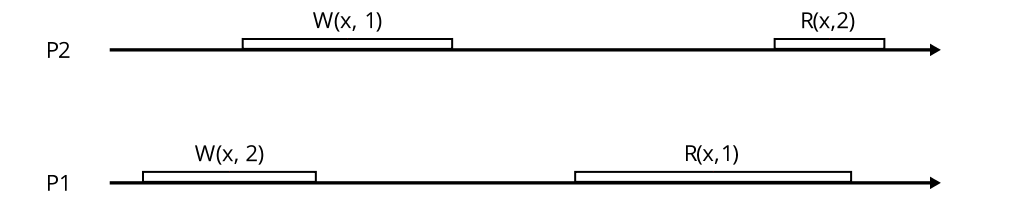
\includegraphics[scale=0.4]{images/causal1.png}
  \caption{A causally consistent, non-sequentially-consistent execution}
\end{figure}

\begin{lemma}
    Sequential consistency implies causal consistency.
\end{lemma}
\begin{proof}
This is immediate from the definitions. Sequential consistency
requires all processes to observe the same total order of events,
where this total order must respect program order. Causal consistency
only requires processes to agree on events that are potentially
causally related. Program order is a subset of causal order, so any
sequential executions also respects causal order.
\end{proof}

However, causal consistency is not nearly as strong as sequential
consistency, as processes do not need to agree on the order of events
with no causal relation between them. This weakness is evident in the
fact that the CAP theorem does not rule out highly available systems
that maintain causal consistency even during network partitions.

\begin{lemma}
    A causally consistent system need not be unavailabile during partitions.
\end{lemma}
\begin{proof}

Suppose $P_1$ and $P_2$ maintain replicas of a key-value store, as
before, and suppose they are separated by a partition. The strategy is
simple: each process immediately handles read requests by reading from
its local replica, and handles write requests by applying the update
to its local replica. It is easy to see this leads to causally
consistent histories. Intuitively, the fact that no information flows
between the processes also means the events of each process are not
related by causality, so causality is not violated.  \end{proof}

Note that in this scenario, a client's requests are always routed to the
same processor. If a client's requests can be routed to any node, causal
consistency cannot be maintained without losing availability. One
sometimes says that causal consistency is ``sticky available'' because
clients must stick to the same processor during partitions.

The fact that causal consistency can be maintained during partitions
suggests it is too weak. Indeed, there are no guarantees about the
difference in values for \(x\) and \(y\) across the two replicas.

\begin{definition}
    FIFO consistency. This also called \emph{pipelined random access memory} or PRAM.
\end{definition}

It is easy to see that causal consistency already implies FIFO
consistency. Figure REF demonstrates that the reverse need not hold. As
a weaker model, FIFO consistency cannot bound the divergence between two
replicas of a data object.

\hypertarget{networks-for-civil-emergency-response}{%
\section{Networks for Civil Emergency
Response}\label{networks-for-civil-emergency-response}}

\hypertarget{physical-communications}{%
\subsubsection{Physical communications}\label{physical-communications}}

The details of the physical communication between processes is outside
the scope of this memo. We make just a few high-level observations about
the possibilities, as the details of the network layer are likely to
have an impact on distributed applications, such as the shared memory
abstraction we discuss below and in Section \ref{sec:contcons}. For such
applications, it may be important to optimize for the sorts of usage
patterns encountered in real scenarios, which are affected by (among
other things) the low-level details of the network.

The \emph{celluar} model (Figure \ref{fig:centralized}) assumes nodes
are within range of a powerful, centralized transmission station that
performs routing functions. Message passing takes place by transmitting
to the base station (labeled \(R\)), which routes the message to its
destination. Such a model could be supported by the ad-hoc deployment of
portable cellphone towers transported into the field, for instance.

The \emph{ad-hoc} model (Figure \ref{fig:decentralized}) assumes nodes
communicate by passing messages directly to each other. This requires
nodes to maintain information about things like routing and the
approximate location of other nodes in the system, increasing complexity
and introducing a possible source of inconsistency. However, it may be
more workable given (i) the geographic mobility of agents in our
scenarios (ii) difficult-to-access locations that prohibit setting up
communication towers (iii) the inherent need for system flexibility
during disaster scenarios.

\begin{figure}
     \centering
     \begin{subfigure}[b]{0.48\textwidth}
         \centering
         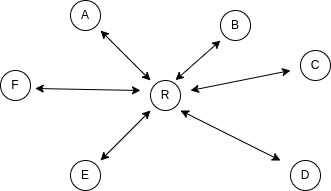
\includegraphics[width=\textwidth]{images/Centralized.png}
         \caption{Cellular network topology}
         \label{fig:centralized}
     \end{subfigure}
     \hfill
     \begin{subfigure}[b]{0.48\textwidth}
         \centering
         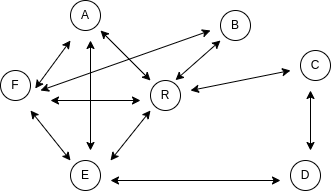
\includegraphics[width=\textwidth]{images/Decentralized.png}
         \caption{Ad-hoc network topology}
         \label{fig:decentralized}
     \end{subfigure}
        \caption{Network topology models for geodistributed agents. Edges represent communication links (bidirectional for simplicity).}
        \label{fig:nettopology}
\end{figure}

One can also imagine hybrid models, such as an ad-hoc arrangement of
localized cells. In general, one expects more centralized topologies to
be simpler for application developers to reason about, but to require
more physical infrastructure and support. On the other hand, the ad-hoc
model is more fault resistant, but more complicated to implement and
potentially offering fewer assurancess about performance. In either
case, higher-level applications such as shared memory abstractions
should be tuned for the networking environment. It would be even better
if this tuning can take place dynamically, with applications
reconfiguring manually or automatically to the particulars of the
operating environment. This requires examining the relationship between
the application and networking layers, rather than treating them as
separate blackboxes.

An interesting possibility is for the \emph{network} to automatically
configure itself to the quality-of-service needs of the application. For
example, a client that receives a lot of requests may be marked as a
preferred client and given higher-priority access to the network. If UAV
vehicles can be used to route messages by acting as mobile transmission
base stations, one can imagine selecting a flight pattern based on
networking needs. For example, if the communication between two
firefighting teams is obstructed by a geographical feature, a UAV could
be dispatched to provide overhead communication support. Such an
arrangement could greatly blur the line between the networking and
application layers.

\hypertarget{desiderata}{%
\section{Desiderata}\label{desiderata}}

\label{sec:des}

Having discussed some of the fundamental distributed systems issues that
arise under real-world network conditions, we turn our attention to
three desiderata we will use to frame and analyze the models discussed
in Sections \ref{sec:contcons} and \ref{sec:sheaf}.

The CAP theorem, and others like it, place fundamental limitations on
the consistency of real-world distributed systems. In the absense of a
``perfect'' system, engineers are forced to make tradeoffs. Ideally,
these tradeoffs should be tuned for the specific application in mind---a
protocol that works well in a datacenter might not work well in a
heterogeneous geodistributed setting. This section lists three desirable
features of distributed systems and frameworks for reasoning about or
implementing them. We chose this set based on the particular details of
civil aviation and disaster response, where safety is a high priority
and usage/communication patterns may be unpredictable.

\hypertarget{d1-quantifiable-bounds-on-inconsistency}{%
\subsubsection{D1: Quantifiable bounds on
inconsistency}\label{d1-quantifiable-bounds-on-inconsistency}}

\emph{A distributed application should quantify the amount of
consistency it delivers. That is, it should (1) provide a mathematical
way of measuring inconsistency between system nodes, and (2) bound
this value while the system is available.}

The CAP theorem implies that an available data replication application
cannot bound inconsistency in all circumstances. When bounded
inconsistency cannot be guaranteed, a system satisfying D1 may become
unavailable. Alternatively, a reasonable behavior would be to continue
providing some form of availability, but alert the user that due to
network and system use conditions the requisite level of consisteny
cannot be guaranteed by the application, leaving the user with the
choice to assess the risk and continue using the system with a weaker
safety guarantees.

\hypertarget{d2-accommodation-of-heterogeneous-nodes}{%
\subsubsection{D2: Accommodation of heterogeneous
nodes}\label{d2-accommodation-of-heterogeneous-nodes}}

\emph{An application should not assume that there is a typical system
node. Instead, the system should accomdate a diverse range of
heterogeneous clients presenting different capabilities, tasks, and
risk-factors.}

One can expect a variety of hardware in the field. For example,
wildfires often involve responses from many different fire departments,
and it must be assumed that they are not always using identical systems.
Different participants in the system may be solving different tasks,
with different levels of access to the network, and they present
different risks. With these sorts of factors in mind, one should hope
for frameworks that are as general as possible to accomodate a wide
variety of clients.

\hypertarget{d3-optimization-for-a-geodistributed-wide-area-network}{%
\subsubsection{D3: Optimization for a geodistributed wide area
network}\label{d3-optimization-for-a-geodistributed-wide-area-network}}

\emph{An application should be optimized for the sorts of
communication patterns that occur in geodistributed wide area networks
(WANs) under real-world conditions.}

Consider two incidents. Wouldn't want to enforce needless global
consistency, particularly if the agents in one area do not have the same
consistency requirements for another area.

Network throughput has some (perhaps approximately linear) relationship
with throughput. Communications patterns are likely far from uniform
too. In fact, these two things likely coincide---it is often that nodes
which are nearby have a stronger need to coordinate their actions than
nodes which are far away. For example, consider manoeauvering airplanes
to avoid crash.

\hypertarget{continuous-consistency-for-shared-memory}{%
\section{Continuous consistency for shared
memory}\label{continuous-consistency-for-shared-memory}}

\label{sec:contcons}

Strong consistency is a discrete proposition: an application provides
strong consistency or it does not. For many real-world applications, it
evidently makes sense to work with data that is consistent up to some
\(\epsilon \in \mathbb{R}^{\geq 0}\). Thus, we shift from thinking about
consistency as an all-or-nothing condition, towards consistency as a
bound on inconsistency.

The definition of \(\epsilon\) evidently requires a more or less
application-specific notion of divergence between replicas of a shared
data object. Take, say, an application for disseminating the most
up-to-date visualization of the location of a fire front. It may be
acceptable if this information appears 5 minutes out of date to a
client, but unacceptable if it is 30 minutes out of date. That is, we
could measure consistency with respect to \emph{time}. One should expect
the exact tolerance for \(\epsilon\) will be depend very much on the
client, among other things. For example, firefighters who are very close
to a fire have a lower tolerance for stale information than a central
client keeping only a birds-eye view of several fire fronts
simultaneously.

Now suppose many disaster-response agencies coordinate with to update
and propagate information about the availability of resources. A client
may want to lookup the number of vehicles of a certain type that are
available to be dispatched within a certain geographic range. We may
stipulate that the value read by a client should always be \(4\) of the
actual number, i.e.~we could measure inconsistency with respect to some
numerical value.

In the last example, the reader may wonder we should tolerate a client
to read a value that is incorrect by 4, when clearly it is better to be
incorrect by 0. Intuitively, the practical benefit of tolerating weaker
values is to tolerate a greater level of imperfection in network
communications. For example, suppose Alice and Bob are individually
authorized to dispatch vehicles from a shared pool. In the event that
they cannot share a message.

Or, would could ask that the the value is a conservative estimate,
possibly lower but not higher than the actual amount. In these examples,
we measure inconsistency in terms of a numerical value.

As a third example,

By varying \(\epsilon\), one can imagine consistency as a continuous
spectrum. In light of the CAP theorem, we should likewise expect that
applications with weaker consistency requirements (high \(\epsilon\))
should provide higher availability, all other things being equal.

Yu and Vahdat explored the CAP tradeoff from this perspective in a
series of papers (Yu and Vahdat 2000a, 2000c, 2000b, 2001, 2002). They
propose a theory of \emph{conits}, a logical unit of data subject to
their three metrics for measuring consistency. By controlling the
threshold of acceptable inconsistency of each conit as a continuous
quantity, applications can exercise precise control the tradeoff between
consistency and performance, trading one for the other in a gradual
fashion.

They built a prototype toolkit called TACT, which allows applications to
specify precisely their desired levels of consistency for each conit. An
interesting aspect of this work is that consistency can be tuned
\emph{dynamically}. This is desirable because one does not know a priori
how much consistency or availability is acceptable.

The biggest question one must answer is the competing goals of
generality and practicality. Generality means providing a general notion
of measuring \(\epsilon\), while practicality means enforcing
consistency in a way that can exploit weakened consistency requirements
to offer better overall performance.

\begin{itemize}
\item
  The tradeoff of CAP is a continuous spectrum between linearizability
  and high-availability. More importantly, it can be tuned in real time.
\item
  TACT captures neither CAP-consistency (i.e.~neither atomic nor
  sequential consistency) nor CAP-availability (read and write requests
  may be delayed indefinitely if the system is unable to enforce
  consistency requirements because of network issues).
\end{itemize}

\hypertarget{tact-system-model}{%
\subsection{TACT system model}\label{tact-system-model}}

As in Section \ref{sec:background}, we assume a distributed set of
processes collaborate to maintain local replicas of a shared data object
such as a database. Processes accept read and write requests from
clients to update items, and they communicate with each other to ensure
to ensure that all replicas remain consistent.

However, access to the data store is mediated by a middleware library,
which sits between the local copy of the replica and the client. At a
high level, TACT will allow an operation to take place if it does not
violate user-specific consistency bounds. If allowing an operation to
proceed would violate consistency constraints, the operation blocks
until TACT synchronizes with one or more other remote replicas. The
operation remains blocked until TACT ensures that executing it would not
violate consistency requirements.

\[\textrm{Consistency} = \langle \textrm{Numerical error, \textrm{Order error}, \textrm{Staleness}} \rangle.\]

Processes forward accesses to TACT, which handles commiting them to the
store. TACT may not immediately process the request---instead it may
need to coordinate with other processes to enforce consistency. When
write requests are processed (i.e.~when a response is sent to the
originating client), they are only commited in a \emph{tenative} state.
Tentative writes eventually become fully committed at some point in the
future, but when they are commited, they may be reordered. After
fullying committing, writes are in a total order known to all processes.

\begin{figure}[h]
  \center
  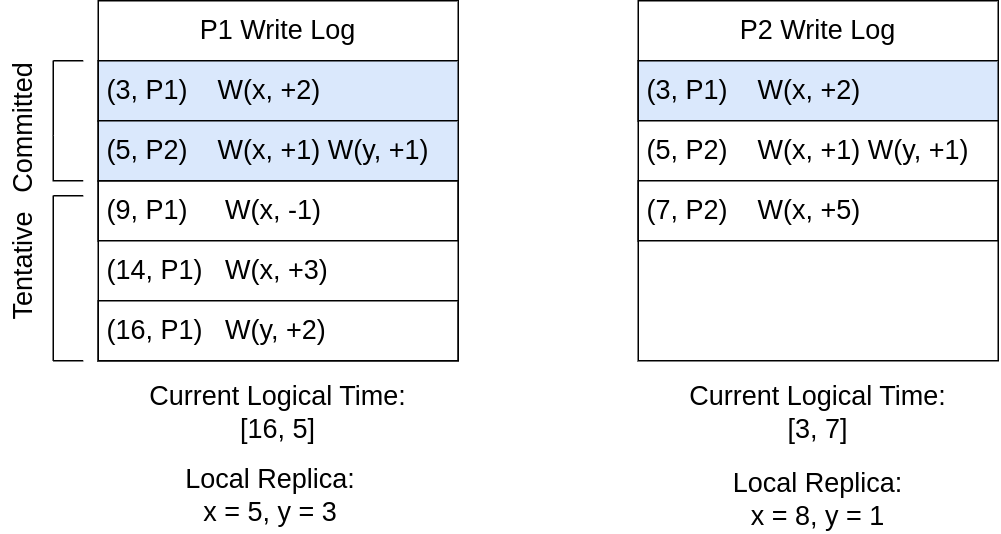
\includegraphics[scale=0.4]{images/TACT Logs.png}
  \caption{Snapshot of two local replicas using TACT}
  \label{fig:tact_logs}
\end{figure}

A write access \(W\) can separately quantify its \emph{numerical weight}
and \emph{order weight} on conit \(F\). Application programmers have
multiple forms of control:

Consistency is enforced by the application by setting bounds on the
consistency of read accesses. The TACT framework then enforces these
consistency levels.

\hypertarget{measuring-consistency-on-conits}{%
\subsection{Measuring consistency on
conits}\label{measuring-consistency-on-conits}}

\hypertarget{numerical-consistency}{%
\paragraph{Numerical consistency}\label{numerical-consistency}}

\hypertarget{order-consistency}{%
\paragraph{Order consistency}\label{order-consistency}}

When the number of tentative (uncommitted) writes is high, TACT executes
a write commitment algorithm. This is a \emph{pull-based} approach which
pulls information from other processes in order to advance \(P_i\)'s
vector clock, raising the watermark and hence allowing \(P_i\) to commit
some of its writes.

\hypertarget{real-time-consistency}{%
\paragraph{Real time consistency}\label{real-time-consistency}}

\hypertarget{enforcing-inconsistency-bounds}{%
\subsection{Enforcing inconsistency
bounds}\label{enforcing-inconsistency-bounds}}

\hypertarget{numerical-consistency-1}{%
\paragraph{Numerical consistency}\label{numerical-consistency-1}}

We describe split-weight AE. Yu and Vahdat also describe two other
schemes for bounding numerical error. One, compound AE, bounds absolute
error trading space for communication overhead. In their simulations,
they found minimal benefits to this tradeoff in general. It is possible
that for specific applications the savings are worth it. They also
consider a scheme, Relative NE, which bounds the relative error.

\hypertarget{order-consistency-1}{%
\paragraph{Order consistency}\label{order-consistency-1}}

\hypertarget{real-time-consistency-1}{%
\paragraph{Real time consistency}\label{real-time-consistency-1}}

\hypertarget{future-work}{%
\subsection{Future work}\label{future-work}}

\hypertarget{integrating-heterogeneous-data}{%
\section{Integrating heterogeneous
data}\label{integrating-heterogeneous-data}}

\label{sec:sheaf}

Strong consistency models provide the abstraction of an idealized global
truth. In the case of conits, the numerical, commit-order, and real-time
errors are measured with respect to an idealized global state of the
database. This state may not exist on any one replica, but it is the
state each replica would converge to if it were to see all remaining
unseen updates.

We consider distributed applications that receive data from many
different sources, such as from a sensor network (broadly defined). It
will often be the case that some sources of data should be expected to
agree with each other, but they may not. A typical scenario, we want to
integrate these data into a larger model of some kind. Essentially take
a poll, and attempt to synthesize a global picture that agrees as much
as possible with the data reported from the sensor network.

Here, we need a consistency model to measure how successful our attempts
are to synthesize a global image. And to tell us how much our sensors
agree. Ideally, we could use this system to diagnose disagreements
between sensors, identifying sensors that appear to be malfunctioning,
or to detect abberations that necessitate a response.

\hypertarget{data-fusion}{%
\subsection{Data fusion}\label{data-fusion}}

To be written.

\hypertarget{presheaves}{%
\subsection{Presheaves}\label{presheaves}}

\begin{definition}
A \emph{partially order-indexed family of sets} is a family of sets indexed by a partially-ordered set,
such that orders between the indices correspond to functions between the sets.
\end{definition}

We can also set \((P, \leq)\) \emph{acts on} the set
\(\{S_i\}_{i \in I}\).

\begin{definition}
A \emph{semiautomaton} is a monoid paired with a set.
\end{definition}

This is also called a \emph{monoid action} on the set.

\begin{definition}
A copresheaf is a *category acting on a family of sets*.
\end{definition}

\begin{definition}
A presheaf is a *category acting covariantly on a family of sets*.
\end{definition}

\hypertarget{sheaves-and-assignments}{%
\subsection{Sheaves and assignments}\label{sheaves-and-assignments}}

To be written.

\hypertarget{the-consistency-radius}{%
\subsection{The consistency radius}\label{the-consistency-radius}}

To be written.

\hypertarget{conclusion}{%
\section{Conclusion}\label{conclusion}}

\label{sec:conclusion}

To be written

\hypertarget{bibliography}{%
\section*{Bibliography}\label{bibliography}}
\addcontentsline{toc}{section}{Bibliography}

\hypertarget{refs}{}
\begin{CSLReferences}{1}{0}
\leavevmode\vadjust pre{\hypertarget{ref-2000brewerCAP}{}}%
Brewer, Eric. 2000. {``Towards Robust Distributed Systems.''} In
\emph{Proceedings of the Nineteenth Annual ACM Symposium on Principles
of Distributed Computing}, 7.
\url{https://doi.org/10.1145/343477.343502}.

\leavevmode\vadjust pre{\hypertarget{ref-2012CAP12Years}{}}%
---------. 2012. {``CAP Twelve Years Later: How the "Rules" Have
Changed.''} \emph{Computer} 45 (2): 23--29.
\url{https://doi.org/10.1109/MC.2012.37}.

\leavevmode\vadjust pre{\hypertarget{ref-10.1145ux2f5505.5508}{}}%
Davidson, Susan B., Hector Garcia-Molina, and Dale Skeen. 1985.
{``Consistency in a Partitioned Network: A Survey.''} \emph{ACM Comput.
Surv.} 17 (3): 341--70. \url{https://doi.org/10.1145/5505.5508}.

\leavevmode\vadjust pre{\hypertarget{ref-1999foxbrewer}{}}%
Fox, A., and E. A. Brewer. 1999. {``Harvest, Yield, and Scalable
Tolerant Systems.''} In \emph{Proceedings of the Seventh Workshop on Hot
Topics in Operating Systems}, 174--78.
\url{https://doi.org/10.1109/HOTOS.1999.798396}.

\leavevmode\vadjust pre{\hypertarget{ref-10.5555ux2f866855}{}}%
Friedman, Roy, and Ken Birman. 1996. {``Trading Consistency for
Availability in Distributed Systems.''} USA: Cornell University.

\leavevmode\vadjust pre{\hypertarget{ref-2002gilbertlynchCAP}{}}%
Gilbert, Seth, and Nancy A. Lynch. 2002. {``Brewer's Conjecture and the
Feasibility of Consistent, Available, Partition-Tolerant Web
Services.''} \emph{SIGACT News} 33 (2): 51--59.
\url{https://doi.org/10.1145/564585.564601}.

\leavevmode\vadjust pre{\hypertarget{ref-2012perspectivesCAP}{}}%
---------. 2012. {``Perspectives on the CAP Theorem.''} \emph{Computer}
45 (02): 30--36. \url{https://doi.org/10.1109/MC.2011.389}.

\leavevmode\vadjust pre{\hypertarget{ref-10.1145ux2f78969.78972}{}}%
Herlihy, Maurice P., and Jeannette M. Wing. 1990. {``Linearizability: A
Correctness Condition for Concurrent Objects.''} \emph{ACM Trans.
Program. Lang. Syst.} 12 (3): 463--92.
\url{https://doi.org/10.1145/78969.78972}.

\leavevmode\vadjust pre{\hypertarget{ref-kshemkalyani_singhal_2008}{}}%
Kshemkalyani, Ajay D., and Mukesh Singhal. 2008. \emph{Distributed
Computing: Principles, Algorithms, and Systems}. Cambridge University
Press. \url{https://doi.org/10.1017/CBO9780511805318}.

\leavevmode\vadjust pre{\hypertarget{ref-2019wideningcap}{}}%
Muñoz-Escoí, Francesc D, Rubén de Juan-Marín, José-Ramón García-Escrivá,
J R González de Mendívil, and José M Bernabéu-Aubán. 2019. {``CAP
Theorem: Revision of Its Related Consistency Models.''} \emph{The
Computer Journal} 62 (6): 943--60.
\url{https://doi.org/10.1093/comjnl/bxy142}.

\leavevmode\vadjust pre{\hypertarget{ref-2017robinsonCanonical}{}}%
Robinson, Michael. 2017. {``Sheaves Are the Canonical Data Structure for
Sensor Integration.''} \emph{Information Fusion} 36: 208--24.
https://doi.org/\url{https://doi.org/10.1016/j.inffus.2016.12.002}.

\leavevmode\vadjust pre{\hypertarget{ref-10.5555ux2f562065}{}}%
Singhal, Mukesh, and Niranjan G. Shivaratri. 1994. \emph{Advanced
Concepts in Operating Systems}. USA: McGraw-Hill, Inc.

\leavevmode\vadjust pre{\hypertarget{ref-TanenbaumSteen07}{}}%
Tanenbaum, Andrew S., and Maarten van Steen. 2007. \emph{Distributed
Systems: Principles and Paradigms}. 2nd ed. Upper Saddle River, NJ:
Pearson Prentice Hall.

\leavevmode\vadjust pre{\hypertarget{ref-2000tact}{}}%
Yu, Haifeng, and Amin Vahdat. 2000a. {``Building Replicated Internet
Services Using TACT: A Toolkit for Tunable Availability and Consistency
Tradeoffs.''} In \emph{Proceedings Second International Workshop on
Advanced Issues of e-Commerce and Web-Based Information Systems. WECWIS
2000}, 75--84. \url{https://doi.org/10.1109/WECWIS.2000.853861}.

\leavevmode\vadjust pre{\hypertarget{ref-10.5555ux2f1251229.1251250}{}}%
---------. 2000b. {``Design and Evaluation of a Continuous Consistency
Model for Replicated Services.''} In \emph{{Proceedings of the 4th
Conference on Symposium on Operating System Design and Implementation -
Volume 4}}. OSDI'00. USA: USENIX Association.

\leavevmode\vadjust pre{\hypertarget{ref-2000tactalgorithms}{}}%
---------. 2000c. {``Efficient Numerical Error Bounding for Replicated
Network Services.''} In \emph{Proceedings of the 26th International
Conference on Very Large Data Bases}, 123--33. VLDB '00. San Francisco,
CA, USA: Morgan Kaufmann Publishers Inc.

\leavevmode\vadjust pre{\hypertarget{ref-DBLP:confux2ficdcsux2fYuV01}{}}%
---------. 2001. {``Combining Generality and Practicality in a
Conit-Based Continuous Consistency Model for Wide-Area Replication.''}
In \emph{Proceedings of the 21st International Conference on Distributed
Computing Systems {(ICDCS} 2001), Phoenix, Arizona, USA, April 16-19,
2001}, 429--38. {IEEE} Computer Society.
\url{https://doi.org/10.1109/ICDSC.2001.918973}.

\leavevmode\vadjust pre{\hypertarget{ref-2002tact}{}}%
---------. 2002. {``Design and Evaluation of a Conit-Based Continuous
Consistency Model for Replicated Services.''} \emph{ACM Trans. Comput.
Syst.} 20 (3): 239--82. \url{https://doi.org/10.1145/566340.566342}.

\end{CSLReferences}

\bibliographystyle{abbrv}
\bibliography{bibliography}
\end{document}
